% DPF 09 talk on strangeness in nucleon

\documentclass[10pt]{beamer}
\usepackage{amsmath}
\usepackage{mathtools}
%\documentclass[12pt]{beamerthemeSam.sty}
\usepackage{epsf}
%\usepackage{pstricks}
%\usepackage[orientation=portrait,size=A4]{beamerposter}
\geometry{paperwidth=160mm,paperheight=120mm}
%DT favorite definitions
\def\LL{\left\langle}	% left angle bracket
\def\RR{\right\rangle}	% right angle bracket
\def\LP{\left(}		% left parenthesis
\def\RP{\right)}	% right parenthesis
\def\LB{\left\{}	% left curly bracket
\def\RB{\right\}}	% right curly bracket
\def\PAR#1#2{ {{\partial #1}\over{\partial #2}} }
\def\PARTWO#1#2{ {{\partial^2 #1}\over{\partial #2}^2} }
\def\PARTWOMIX#1#2#3{ {{\partial^2 #1}\over{\partial #2 \partial #3}} }

\def\rightpartial{{\overrightarrow\partial}}
\def\leftpartial{{\overleftarrow\partial}}
\def\diffpartial{\buildrel\leftrightarrow\over\partial}

\def\BI{\begin{itemize}}
\def\EI{\end{itemize}}
\def\BE{\begin{displaymath}}
\def\EE{\end{displaymath}}
\def\BEA{\begin{eqnarray*}}
\def\EEA{\end{eqnarray*}}
\def\BNEA{\begin{eqnarray}}
\def\ENEA{\end{eqnarray}}
\def\EL{\nonumber\\}


\newcommand{\map}[1]{\frame{\frametitle{\textbf{Course map}}
\centerline{\includegraphics[height=0.86\paperheight]{../../map/#1.png}}}}
\newcommand{\wmap}[1]{\frame{\frametitle{\textbf{Course map}}
\centerline{\includegraphics[width=0.96\paperwidth]{../../map/#1.png}}}}

\newcommand{\etal}{{\it et al.}}
\newcommand{\gbeta}{6/g^2}
\newcommand{\la}[1]{\label{#1}}
\newcommand{\ie}{{\em i.e.\ }}
\newcommand{\eg}{{\em e.\,g.\ }}
\newcommand{\cf}{cf.\ }
\newcommand{\etc}{etc.\ }
\newcommand{\atantwo}{{\rm atan2}}
\newcommand{\Tr}{{\rm Tr}}
\newcommand{\dt}{\Delta t}
\newcommand{\op}{{\cal O}}
\newcommand{\msbar}{{\overline{\rm MS}}}
\def\chpt{\raise0.4ex\hbox{$\chi$}PT}
\def\schpt{S\raise0.4ex\hbox{$\chi$}PT}
\def\MeV{{\rm Me\!V}}
\def\GeV{{\rm Ge\!V}}

%AB: my color definitions
%\definecolor{mygarnet}{rgb}{0.445,0.184,0.215}
%\definecolor{mygold}{rgb}{0.848,0.848,0.098}
%\definecolor{myg2g}{rgb}{0.647,0.316,0.157}
\definecolor{abtitlecolor}{rgb}{0.0,0.255,0.494}
\definecolor{absecondarycolor}{rgb}{0.0,0.416,0.804}
\definecolor{abprimarycolor}{rgb}{1.0,0.686,0.0}
\definecolor{Red}           {cmyk}{0,1,1,0}
\definecolor{Grey}           {cmyk}{.7,.7,.7,0}
\definecolor{Blue}          {cmyk}{1,1,0,0}
\definecolor{Green}         {cmyk}{1,0,1,0}
\definecolor{Brown}         {cmyk}{0,0.81,1,0.60}
\definecolor{Black}         {cmyk}{0,0,0,1}

\usetheme{Madrid}


%AB: redefinition of beamer colors
%\setbeamercolor{palette tertiary}{fg=white,bg=mygarnet}
%\setbeamercolor{palette secondary}{fg=white,bg=myg2g}
%\setbeamercolor{palette primary}{fg=black,bg=mygold}
\setbeamercolor{title}{fg=abtitlecolor}
\setbeamercolor{frametitle}{fg=abtitlecolor}
\setbeamercolor{palette tertiary}{fg=white,bg=abtitlecolor}
\setbeamercolor{palette secondary}{fg=white,bg=absecondarycolor}
\setbeamercolor{palette primary}{fg=black,bg=abprimarycolor}
\setbeamercolor{structure}{fg=abtitlecolor}

\setbeamerfont{section in toc}{series=\bfseries}

%AB: remove navigation icons
\beamertemplatenavigationsymbolsempty
\title[Problem solving: kinematics]{
  \textbf {Problem solving: kinematics (II)}\\
%\centerline{}
%\centering
%\vspace{-0.0in}
%\includegraphics[width=0.3\textwidth]{propvalues_0093.pdf}
%\vspace{-0.3in}\\
%\label{intrograph}
}

\author[W. Freeman] {Physics 211\\Syracuse University, Physics 211 Spring 2015\\Walter Freeman}

\date{\today}

\begin{document}

\frame{\titlepage}

\frame{\frametitle{\textbf{Announcements}}
\BI
\item{Homework 2 due date is {\bf extended until Friday}}
\item{Bring your clicker and/or ResponseWare app on Thursday}
\item{Around 25 people in the Clinic during my office hours today}
\item{The course schedule is available on the wiki}
\item{Exam 1 is next Tuesday}
  \BI
\item{No homework due next week}
\item{Sample exam will be posted today}
  \EI

\EI
}

\frame{\frametitle{\textbf{Exam 1}}
 \BI
 \item{The exam covers kinematics in one and two dimensions}
 \item{Kinematics: how are an object's position, velocity, and acceleration related?}
   \pause
 \item{\color{Red}The exam will be substantially easier than the homework.}
   \pause
 \item{You may use a scientific (not graphing) calculator on the exam.}
 \item{Bring: your calculator, pencils, and your physics smarts (frog optional)}
   \pause
\item{Formal review session in class on Thursday}
  \BI
\item{At this review you will create your reference sheet, which I will post in final form that day}
  \EI
\item{Other review times TBA (poll)}
 \EI
}

\frame{\frametitle{\textbf{Exam 1, promises}}
  \BI
\item{There will be one problem where you need the quadratic formula}
  \BI
\item{... this means interpreting the two values it spits out}
  \EI
\item{There will be at least one instance where you need to graph position, velocity, and acceleration}
\item{You will {\it not} need to compute derivatives or integrals algebraically}
  \EI
}


\frame{\frametitle{\textbf{Last time}}

    \large Acceleration, velocity, and position relationships are the same in 2D; they just apply {\color{Red}independently} for each component.
    \Large

    \begin{align*}
      \vec v(t) =&\, \vec at + \vec v_0 \\
      \vec r(t) =&\, \frac{1}{2}\vec a t^2 + \vec v_0 t + \vec r_0
    \end{align*}

    \pause

    \begin{align*}
      \vec v_x(t) =&\, a_x t + v_{x,0} \\
      \vec v_y(t) =& a_y t + v_{y,0} \\
    \end{align*}
    \pause
    \begin{align*}
      \vec x(t) =&\,  \frac{1}{2}  a_x t^2 + v_{x,0} t + x_0\\
      \bigskip
      \vec y(t) =&\, \frac{1}{2}  a_y t^2 + v_{y,0} t + y_0
    \end{align*}
  }
   \frame{\frametitle{\textbf{Working with variables}}
    \Large 
    \centerline{If you don't know the numerical value of a quantity yet, }
      \centerline{it's fine to leave it as a variable!}

    \bigskip

    \centerline{This is essential for solving many problems.}

    \pause

\bigskip
\bigskip

\centerline{Example from cannon problem:}

\begin{eqnarray*}
  x(t) = \frac{1}{2} a_x t^2 + {\color{Red}v_{x,0}} t + x_0 \\
  y(t) = \frac{1}{2} a_y t^2 + {\color{Red}v_{y,0}} t + y_0 
\end{eqnarray*}
}


   \frame{\frametitle{\textbf{Working with variables}}
    \Large 
  \centerline{If you don't know the numerical value of a quantity yet, }
      \centerline{it's fine to leave it as a variable!}

    \bigskip

    \centerline{This is essential for solving many problems.}



\bigskip
\bigskip

\centerline{Example from cannon problem:}

\begin{align*}
  x(t) =& {\color{Red}v_{x,0}} t \\
    y(t) =& -\frac{1}{2} g t^2 + {\color{Red}v_{y,0}} t 
  \end{align*}


}




   \frame{\frametitle{\textbf{Working with variables}}
    \Large 
  \centerline{If you don't know the numerical value of a quantity yet, }
      \centerline{it's fine to leave it as a variable!}

    \bigskip

    \centerline{This is essential for solving many problems.}



\bigskip
\bigskip

\centerline{Example from cannon problem:}

\begin{align*}
  x(t) =& {\color{Red}v_0 \cos 45^o} t \\
  y(t) =& -\frac{1}{2} g t^2 + {\color{Red}v_0 \sin 45^o} t \\
\end{align*}

  \centerline{(I leave the rest to you for now...)}

}



  \frame{\frametitle{\textbf{Problem solving: 2D kinematics, constant acceleration}}
    \large
    \begin{enumerate}
      \item{1. If you have vectors in the ``angle and magnitude'' form ($\vec a, \vec v, \vec r$), convert them to components}
      \item{2. Write down the kinematics relations, separately for $x$ and $y$}
        \begin{itemize}
            \large
          \item{Many terms will usually be zero}
          \item{Freefall: $a_x = 0$, $a_y = -g$ (with conventional choice of axes)}
        \end{itemize}
      \item{3. Understand what instant in time you want to know about}
      \item{4. Put in what you know; solve for what you don't (using substitution, if necessary)}
      \item{5. Think about the physical meaning of your solution}
    \end{enumerate}
  }


  \frame{\frametitle{\textbf{Problem solving: 2D kinematics, constant acceleration}}
    \large
    \begin{enumerate}
      \item{1. If you have vectors in the ``angle and magnitude'' form ($\vec a, \vec v, \vec r$), convert them to components}
      \item{2. Write down the kinematics relations, separately for $x$ and $y$}
        \begin{itemize}
            \large
          \item{Many terms will usually be zero}
          \item{Freefall: $a_x = 0$, $a_y = -g$ (with conventional choice of axes)}
        \end{itemize}
      \item{{\color{Red}3. Understand what instant in time you know about (or want to know about)}}
      \item{4. Put in what you know; solve for what you don't (using substitution, if necessary)}
      \item{5. Think about the physical meaning of your solution}
    \end{enumerate}
  }

  \frame{\frametitle{\textbf{``What instant in time do you know about?''}}
  \large
  This is often the most difficult part of problems: it requires thought, not just math.

  \bigskip

  \BI
\item{``Object strikes (level) ground'': often means y=0, if that is where your ground is}
  \pause
\item{``Object reaches maximum height'': usually means $v_y=0$}
  \pause
\item{``Two objects meet'': $x_1 = x_2, y_1 = y_2$ at the same time (frog/spider, cat/cheeseburger problems)}
  \EI
}




\frame{\frametitle{\textbf{A cannon}}
\large
\BI
\item{A cannon shoots a cannonball at 80 $m/s$ at an angle of 30 degrees above the horizontal.}
\item{If the cannon is on level ground, how far does the cannonball go?}
  \pause
\item{How high does the cannonball go?}
  \pause
\item{How fast is it traveling at its highest point?}
  \pause
\item{How fast is it traveling when it strikes the ground?}
  \EI
}


\frame{\frametitle{\textbf{A cannon}}
\large
\BI
\item{A cannon shoots a cannonball at initial velocity $v_0$ at an angle $\theta$ above the horizontal.}
\item{If the cannon is on level ground, how far does the cannonball go?}
  \pause
\item{How high does the cannonball go?}
\pause
\item{How fast is it traveling at its highest point?}
  \pause
\item{How fast is it traveling when it strikes the ground?}
  \EI

\bigskip
\bigskip
\centerline{Note that this algebraic solution can be used to do other things rather simply!}

}


\frame{\frametitle{\textbf{Throwing a rock off a cliff}}
  \BI
\item{A hiker throws a rock horizontally off of a 100m tall cliff. If the rock strikes the ground 30m away, how hard did she 
  throw it? How fast was it going when it hit the ground?}
  \pause
 
\item { Write down the basic position relations (terms that are zero in red):}

  $x(t) = {\color{Red} \frac{1}{2} a_xt^2} + v_{0,x} t + \color{Red}x_0$
  
 $y(t) = {\frac{1}{2} a_yt^2} + {\color{Red}v_{0,y}} t + y_0$
  
  \pause

\item{The first one gives us a very simple relationship between the horizontal distance $d$ travelled and the time the rock takes to fall:}
 $d = v_0 t$
\pause

\item{We can find the time it takes to fall from the $y$ equation:  }

  $0 = \frac{1}{2} (-g)t^2 + h$
  
  \pause
 
\item{Now we just do some algebra:}
  
$t = \sqrt{\frac{2h}{g}}$

  \pause

$d = v_0 \sqrt{\frac{2h}{g}} \rightarrow v_0 = 30 \sqrt{\frac{9.8}{100\cdot2}}=6.64$ m/s

\pause

\item{  To get the speed when it hits, we just use the velocity relations:}
\item{$v_x = v_{0,x}$ and $v_y = -gt$}
\item{$v_x = 6.64$ m/s, $v_y = \sqrt{2gh} = -44.2$ m/s}
\item{$|v| = \sqrt{v_x^2 + v_y^2} = 44.7$ m/s}
\EI
      }

      \frame{\frametitle{\textbf{The roadrunner problem}}
\large
The position of the car is given by the ordinary 1D kinematics relation:

\bigskip

$x(t) = \frac{1}{2} at^2 + v_0 t = \frac{1}{2} (-9) t^2 + (30.6) t$ (mks units)

\pause
\bigskip

We care about the time when it meets up with the position of the roadrunner, which is 30m. So we set $x(t) = 30$ and solve.

\centerline{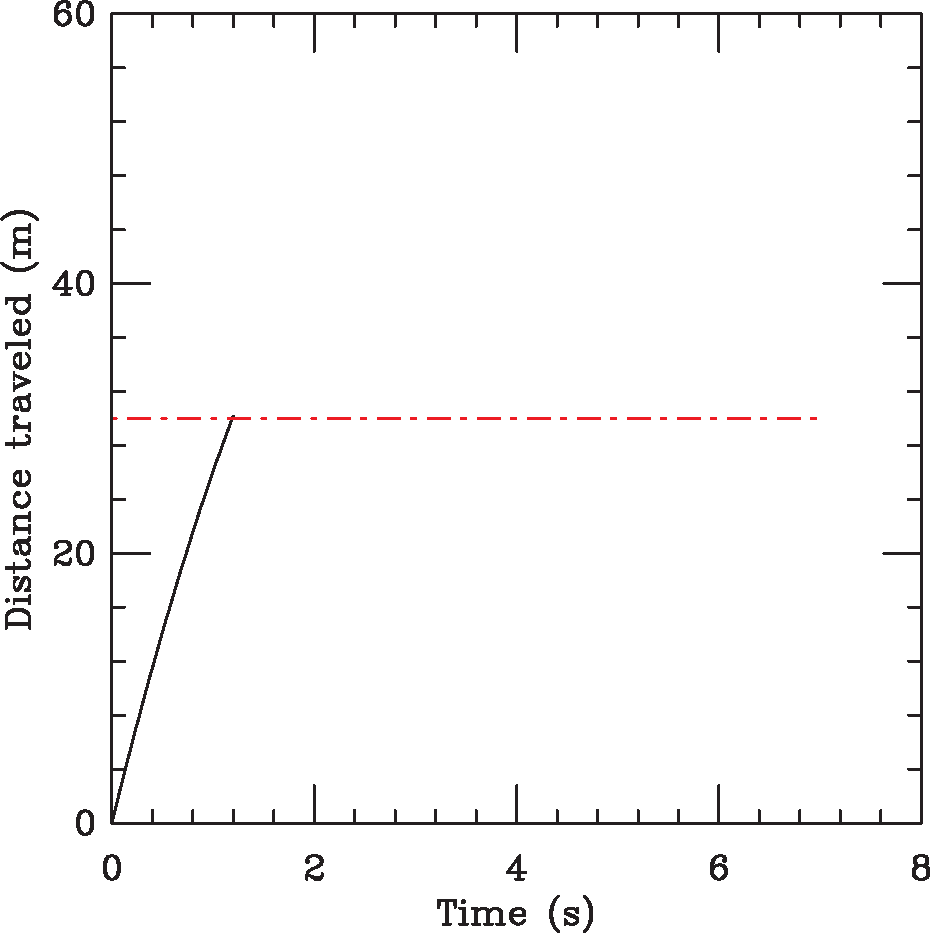
\includegraphics[width=0.3\textwidth]{rr1-crop.pdf}}

This seems easy enough, but the quadratic formula gives us two solutions! What happened?

}

\frame{\frametitle{\textbf{The roadrunner problem}}
\large
The position of the car is given by the ordinary 1D kinematics relation:

\bigskip

$x(t) = \frac{1}{2} at^2 + v_0 t = \frac{1}{2} (-9 m/s^2) t^2 + (30.6 m/s) t$

\bigskip

We care about the time when it meets up with the position of the roadrunner, which is 30m. So we set $x(t) = 30$ and solve.

\centerline{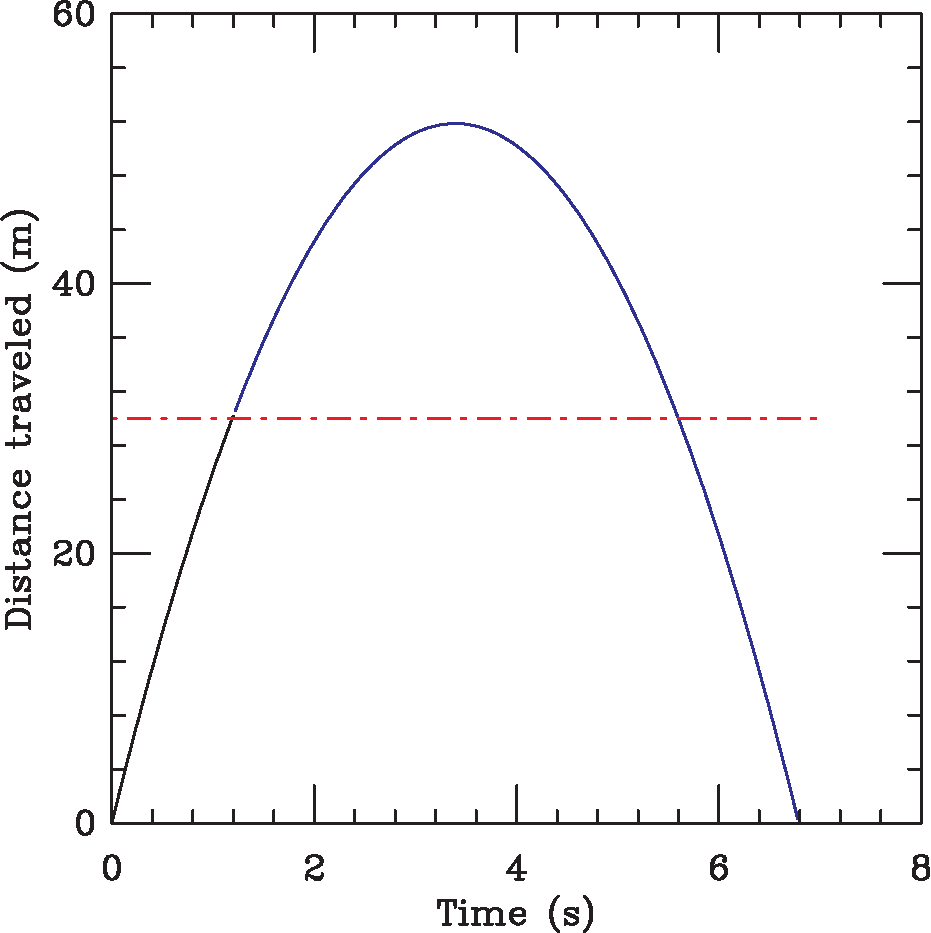
\includegraphics[width=0.3\textwidth]{rr2-crop.pdf}}

\pause

Moral of the story: mathematics is a very blunt tool!

}


\frame{\frametitle{\textbf{Throwing a stone onto a slope}}
  A hiker kicks a stone off of a mountain slope with an initial velocity of 3 m/s horizontally. If the mountain has a slope
  of 45 degrees, how far down the slope does it land?

  \pause
\BI
\item{  Same kinematic relations as before (this is always a good starting point!)}


 $x(t) = {\color{Red} \frac{1}{2} a_xt^2} + v_{0,x} t + \color{Red}x_0$
  
 $y(t) = {\frac{1}{2} a_yt^2} + {\color{Red}v_{0,y}} t + y_0$

\bigskip
\pause

\item{Now the condition for ``rock hits ground'' requires some thought:}
\pause
\item{The rock hits the ground when $x(t)=-y(t)$}

  
  $v_{0,x}t=\frac{1}{2}gt^2 \rightarrow t=\frac{2v_{0,x}}{g}$

  \pause
\item{This gives us $x(t) = \frac{2v_{0,x}^2}{g}$}
\item{$y(t)$ will have the same magnitude: the Pythagorean theorem gives $|r| = 2 \sqrt{2} \frac{v_{0,x}^2}{g}$}
\EI
}

  
\frame{\frametitle{\textbf{A rocket}}
 \Large
  A rocket is launched from rest on level ground. While its motor burns, it accelerates at 10 m/s at an angle 30 degrees
  below the vertical. After ten seconds its motor burns out and it follows a ballistic trajectory until it hits the ground.

  \bigskip

  How far does it go?

}


      \end{document}
